\documentclass[conference]{IEEEtran}
\IEEEoverridecommandlockouts

\usepackage{amsmath,amssymb}
\usepackage{graphicx}
\usepackage{booktabs}
\usepackage{cite}
\usepackage{url}
\usepackage[hidelinks]{hyperref}

\graphicspath{{figs/}}

% let floats pack pages tightly (4-page limit)
\renewcommand{\topfraction}{0.92}
\renewcommand{\bottomfraction}{0.85}
\renewcommand{\textfraction}{0.06}
\renewcommand{\floatpagefraction}{0.75}
\setcounter{topnumber}{3}
\setcounter{totalnumber}{4}

\begin{document}

\title{Zero-Shot Monocular Depth Estimation for Metric Object Sizing in
Low-Contrast Environments}

\author{
\IEEEauthorblockN{Huang JunLin}
\IEEEauthorblockA{School of Engineering\\
Nanyang Polytechnic\\
Singapore}
}

\maketitle

\begin{abstract}
We ask how far a purely zero-shot pipeline can go from a single RGB image to
tape-measured object dimensions. The pipeline pairs a frozen YOLOv8m detector
with a frozen monocular depth model and converts relative depth into metres with
a two-anchor disparity fit; a pinhole back-projection then yields each object's
distance $Z$, width $W$ and height $H$. On a purpose-built 100-image dataset
(five household objects, five distances from 0.50 to 0.90~m, four lighting
conditions including an active-infrared night mode) we benchmark five depth
backbones: Depth Anything V2 Small/Base/Large, MiDaS (DPT-Hybrid) and Marigold.
Depth Anything V2 Large is best, with 3.63~cm mean absolute distance error
(4.9\,\%), 9.3\,\% / 4.9\,\% relative width / height error and no gross failures,
against 9.38~cm for MiDaS. The aggregate hides a strongly non-uniform error
profile: 61\,\% of the total absolute distance error comes from one tall, thin,
clear bottle, and that error is a one-directional over-estimation almost
entirely explained by where depth is sampled inside the box; sampling the
ground-contact point instead of the box interior cuts it by 40\,\% at no cost.
Night-time infrared capture is the second failure mode, and its error tracks
highlight clipping rather than low contrast. We also show that 5\,\% of
detection rows must be voided rather than scored, and that scoring them silently
can roughly double a model's reported error.
\end{abstract}

\begin{IEEEkeywords}
monocular depth estimation, zero-shot inference, object sizing, YOLO,
geometric calibration, benchmark
\end{IEEEkeywords}

\section{Introduction}
Turning a photograph into a physical measurement recurs in agriculture,
logistics, inventory and robotic manipulation: a system that reports ``this fruit
is 7.4~cm across and 62~cm away'' from the camera it already has needs no depth
sensor, no stereo rig and no calibration target on the object. Monocular depth
estimation (MDE) is strong in the zero-shot regime~\cite{ranftl2022midas,yang2024dav2},
but published benchmarks report relative-depth metrics on internet-scale imagery,
not centimetres on a tableside object under a dim bulb. This paper asks: \emph{if
we freeze a detector and a depth model and bolt a two-anchor calibration onto
them, how accurate are the resulting metric dimensions, and where does that
accuracy break?}

We answer with a 100-image capture matrix that isolates object identity, distance
and illumination on a locked-down rig, with every distance and object dimension
tape-measured. Every model is used as shipped: no fine-tuning, no per-scene
optimisation, no test-time adaptation. Our contributions are:

\begin{itemize}
\item a reproducible zero-shot pipeline that converts detector boxes plus
relative depth into per-object $Z$, $W$ and $H$ (Section~\ref{sec:method}), with
a 100-image dataset spanning lighting, distance and object axes;
\item a five-model benchmark on that dataset, reported in aggregate and
decomposed by lighting, distance and object (Section~\ref{sec:results});
\item the finding that the aggregate error is dominated by a single object
geometry, that this error is a signed bias rather than noise, and that a
one-line change to depth sampling removes 40\,\% of it
(Section~\ref{sec:b01});
\item an evaluation-integrity result: without a detection gate, 10\,\% of rows
silently size the wrong object and inflate reported error by up to
2$\times$ (Section~\ref{sec:integrity}).
\end{itemize}

\section{Related Work}
Eigen \emph{et al.}~\cite{eigen2014depth} established single-image depth
regression; MiDaS~\cite{ranftl2022midas,ranftl2021dpt} scaled it and made
cross-dataset zero-shot transfer the norm. Depth Anything
V1/V2~\cite{yang2024da,yang2024dav2} extend that recipe with large-scale
unlabelled data, while Marigold~\cite{ke2024marigold} re-casts depth as
conditional diffusion on a pretrained image generator. All of these predict
\emph{relative} or affine-invariant depth, so calibration is unavoidable for
metrology; metric variants (ZoeDepth~\cite{bhat2023zoedepth},
Metric3D~\cite{yin2023metric3d}) are tied to the camera and domain of their
training data, which is what a plug-and-play deployment avoids.

We take object extents from YOLO~\cite{redmon2016yolo} in its Ultralytics
form~\cite{jocher2023yolov8}. Boxes are the cheapest localisation available and
their tightness becomes a first-order error term for thin objects
(Section~\ref{sec:results}). Back-projecting pixels through a pinhole model is
textbook geometry~\cite{hartley2004mvg}; the open question is the depth stage
feeding it. Existing benchmarks (KITTI~\cite{geiger2012kitti},
NYU-Depth~\cite{silberman2012indoor}) use LiDAR or RGB-D ground truth in driving
or room scenes and report scale-invariant errors, so they do not answer how a
commodity camera with an assumed field of view performs on small objects at
0.5--0.9~m under warm, dim and infrared light.

\begin{figure*}[t]
\centering
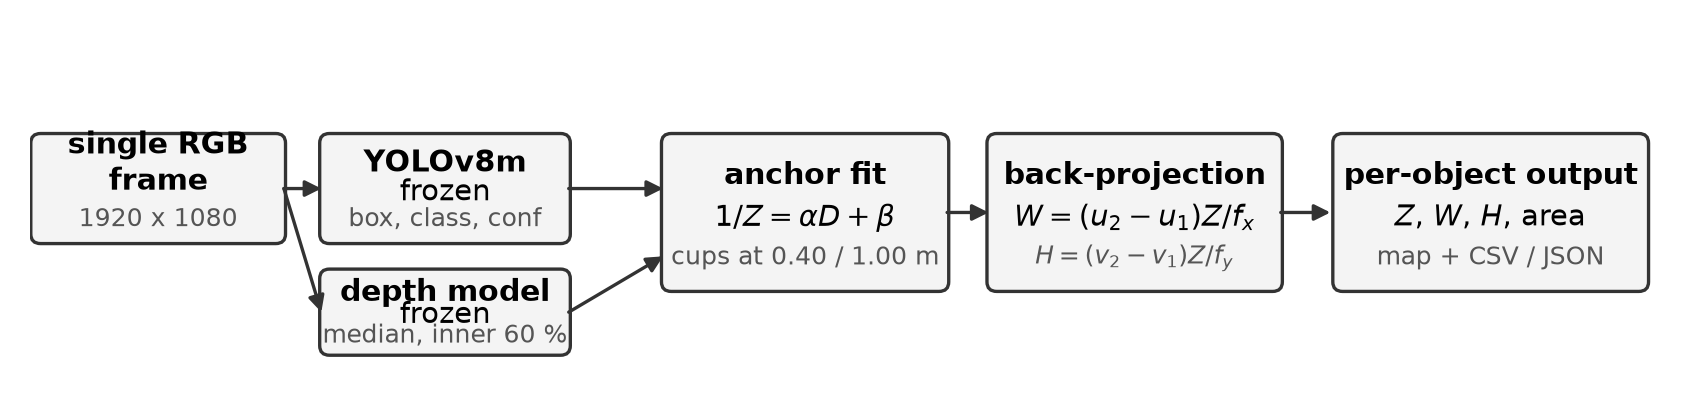
\includegraphics[width=\textwidth]{fig1_pipeline.png}
\caption{The pipeline. Both learned components are frozen. Detections are gated
to the expected class, the depth map is sampled inside each surviving box, and a
two-anchor least-squares fit in disparity space maps relative depth to metres
before the pinhole back-projection produces $Z$, $W$ and $H$.}
\label{fig:pipeline}
\end{figure*}

\section{Method}
\label{sec:method}

\subsection{Overview}
Figure~\ref{fig:pipeline} shows the five stages. A 1920$\times$1080 RGB frame
goes to YOLOv8m, which returns boxes, classes and confidences, while a frozen
depth model returns a dense relative-depth map $D$. Each surviving box selects a
scalar depth statistic, the anchors calibrate it to metres, and the pinhole model
turns the box extent at that depth into physical width and height, one row per
object.

\subsection{Disparity-Domain Anchor Calibration}
Let $D(u,v)$ be the raw model output. The natural alignment is linear in depth,
\begin{equation}
Z(u,v) = \alpha\,D(u,v) + \beta ,
\label{eq:affine}
\end{equation}
with $(\alpha,\beta)$ fitted by least squares to tape-measured distances.
Relative-depth models, however, are trained against \emph{inverse} depth, so $D$
behaves like disparity and fitting \eqref{eq:affine} warps any object lying
between the calibration anchors. We instead fit
\begin{equation}
\frac{1}{Z(u,v)} = \alpha\,D(u,v) + \beta
\quad\Longrightarrow\quad
Z(u,v) = \frac{1}{\alpha\,D(u,v) + \beta},
\label{eq:inverse}
\end{equation}
which is exact for a model whose output is proportional to disparity and
interpolates correctly between anchors. Both forms are implemented; all results
here use \eqref{eq:inverse}.

Two physical reference cups are placed at known distances, 0.40~m and 1.00~m, in
every scene and clicked once per scene folder, so calibration costs two clicks
and no per-object measurement. The anchors bracket the working range
(0.50--0.90~m), so the object always lies between them.

\subsection{Depth Sampling and Back-Projection}
A box covers a surface patch, not a point, so a scalar depth must be chosen. Our
default takes the median of $D$ over the interior 60\,\% of the box, which is
robust to stray background pixels; Section~\ref{sec:b01} shows this is the wrong
choice for tall, thin objects and evaluates alternatives. Given $Z$ at the object
and focal lengths $(f_x,f_y)$, the pinhole model gives
\begin{equation}
W = \frac{|u_2-u_1|\,Z}{f_x}, \qquad
H = \frac{|v_2-v_1|\,Z}{f_y},
\label{eq:size}
\end{equation}
for a box spanning $u_1..u_2$ and $v_1..v_2$. Intrinsics come from EXIF when
available; this camera reported nothing usable, so we assume a 65$^\circ$
horizontal field of view, giving $f_x=f_y=1506.9$~px. That assumption scales all
absolute numbers uniformly and is revisited in Section~\ref{sec:limits}.

\subsection{Detection Gating and Row Voiding}
An early version scored whatever detection was most confident between the two
anchors. Since the anchors are themselves cups, that frequently scored a
\emph{calibration cup}, a knife or the table, and because ground-truth distance
comes from the filename the resulting ``errors'' were 10--50~cm of pure
bookkeeping (Section~\ref{sec:integrity}). The pipeline now applies three rules:
(i) drop any detection whose box contains an anchor click, which is exact because
the clicks land on the anchor cups; (ii) keep only detections of the class the
scene is about, from the object id or a target flag; (iii) if none survives, void
the row instead of scoring it. Voided rows are logged, excluded from every
metric, and counted in the summary.

\section{Experimental Setup}

\subsection{Dataset and Rig}
The dataset contains 100 images: five objects $\times$ five distances (0.50 to
0.90~m in 10~cm steps) $\times$ four lighting conditions. The objects, with
tape-measured $W\times H$, are a bowl (12.0$\times$6.0~cm), a mug
(12.0$\times$8.0~cm), an apple (7.5$\times$7.0~cm), a short, blue,
translucent bottle (7.5$\times$25.0~cm) and a tall, narrow, clear
bottle (6.2$\times$24.0~cm). The lighting modes are \emph{white}, evenly lit and used as
reference; \emph{warm}, a strong yellow cast; \emph{dim}, low and flat; and
\emph{nv}, lights off with an active-infrared illuminator, producing a
near-monochrome frame. The camera is locked on a tripod and no capture parameter
changes. The two reference cups sit at 0.40~m and 1.00~m in every scene and the
measured object is placed at the target distance with a tape measure. One image
per cell, so the design measures systematic behaviour, not shot-to-shot
variance.

\subsection{Models and Implementation}
We benchmark five frozen backbones: Depth Anything V2 Small, Base and Large (the
\texttt{-hf} Transformers checkpoints)~\cite{yang2024dav2}; MiDaS in its
DPT-Hybrid form~\cite{ranftl2022midas,ranftl2021dpt}; and
Marigold~\cite{ke2024marigold}. Detection is YOLOv8m~\cite{jocher2023yolov8} at
confidence 0.25 for every model. All five see identical boxes, anchors and
calibration, with box-median depth sampling. Runs used one RTX 4070 (12~GB).
Five models times 100 images gives 500 (model, image) pairs, of which 475 are
scored and 25 voided.

\subsection{Metrics}
For each scored row we report $|\hat Z - Z|$ and $|\hat Z - Z|/Z$ and derive MAE,
RMSE, mean signed bias and the fraction exceeding 20~cm or 30\,\%. Sizing accuracy is mean absolute relative error of $W$ and of $H$ against
the tape-measured table.

\begin{table}[t]
\centering
\caption{Overall accuracy over 475 scored rows per model (25 voided rows
excluded). Bias is the mean signed error; $>$20~cm and $>$30\,\% are gross-failure
rates. Best value in each column is bold.}
\label{tab:overall}
\footnotesize
\setlength{\tabcolsep}{3.5pt}
\begin{tabular}{lcccccccc}
\toprule
Model & MAE & rel & bias & RMSE & $>$20 & $>$30 & $W$ & $H$\\
      & (cm) & (\%) & (cm) & (cm) & (cm) & (\%) & (\%) & (\%)\\
\midrule
DA-V2-S & 5.78 & 8.0 & $+4.77$ & 10.71 & 12 & 7 & 12.9 & 8.3\\
DA-V2-B & 5.35 & 7.4 & $+4.99$ & 7.83 & 5 & 1 & 11.8 & 6.1\\
\textbf{DA-V2-L} & \textbf{3.63} & \textbf{4.9} & $+3.21$ & \textbf{5.15} &
\textbf{0} & \textbf{0} & \textbf{9.3} & \textbf{4.9}\\
MiDaS & 9.38 & 13.1 & $+5.26$ & 15.91 & 12 & 12 & 15.5 & 11.1\\
Marigold & 8.55 & 12.1 & $-3.12$ & 11.62 & 3 & 2 & 14.3 & 13.5\\
\bottomrule
\end{tabular}
\end{table}

\section{Results and Discussion}
\label{sec:results}

\subsection{Overall Accuracy}
Depth Anything V2 Large wins every column of Table~\ref{tab:overall}: 3.63~cm MAE
(4.9\,\%), 5.15~cm RMSE, 9.3\,\% width and 4.9\,\% height error, and no detection
beyond 20~cm or 30\,\%. Its RMSE sits close to its MAE, so errors are small and
evenly spread; Small's RMSE is nearly twice its MAE (10.71 vs 5.78~cm), meaning a
few rows drive it, and that fragility rather than the mean is the real difference
between the sizes. Base is a defensible middle ground. Accuracy is monotone in
model size within the family, and the family beats both baselines on distance
\emph{and} sizing. MiDaS (9.38~cm) is weakest overall; Marigold lands at 8.55~cm at
diffusion-sampling cost (Section~\ref{sec:limits}).

Every model except Marigold over-estimates distance, with mean $\hat Z/Z$ of
1.062 (Small), 1.067 (Base), 1.042 (Large) and 1.075 (MiDaS); Marigold
under-estimates at 0.949. One multiplicative correction fitted on the anchors
would recover 4--7 points of relative error for free, and would improve $W$ and
$H$ in proportion since both scale linearly with $Z$.

\begin{table}[t]
\centering
\caption{MAE of $Z$ in cm / mean relative error in \%, by lighting condition
(rows 1--4) and by object (rows 5--9). The apple has $n=15$ per model and the
\emph{nv} rows $n=20$, because the apple is never detected at night. Marigold is
omitted here and discussed in the text.}
\label{tab:groups}
\footnotesize
\setlength{\tabcolsep}{4pt}
\begin{tabular}{lcccc}
\toprule
Condition & DA-V2-S & DA-V2-B & DA-V2-L & MiDaS\\
\midrule
\multicolumn{5}{l}{\emph{by lighting}}\\
dim    & 4.47 / 6.1  & 4.66 / 6.3  & \textbf{2.90 / 3.9} & 5.42 / 8.0\\
white  & 4.45 / 6.1  & 4.73 / 6.5  & 3.42 / 4.5 & 12.32 / 17.1\\
warm   & 5.16 / 7.2  & 5.08 / 7.1  & 3.72 / 5.1 & 6.93 / 10.1\\
nv     & 9.84 / 13.9 & 7.33 / 10.3 & 4.69 / 6.6 & 13.73 / 18.3\\
\midrule
\multicolumn{5}{l}{\emph{by object}}\\
bowl   & \textbf{1.23 / 1.9} & 1.73 / 2.3 & 1.67 / 2.2 & 7.13 / 9.0\\
mug    & 2.42 / 3.5 & 1.43 / 2.2 & \textbf{1.21 / 1.8} & 3.77 / 5.1\\
apple  & \textbf{1.57 / 2.2} & 2.95 / 3.9 & 2.37 / 3.1 & 4.63 / 6.7\\
bottle, short & \textbf{2.49 / 3.6} & 6.17 / 8.4 & 3.73 / 4.8 & 20.23 / 29.0\\
bottle, tall  & 20.12 / 27.3 & 13.89 / 19.4 & \textbf{8.86 / 12.4} & 9.97 / 14.2\\
\bottomrule
\end{tabular}
\end{table}

\subsection{Effect of Lighting}
Table~\ref{tab:groups} overturns the intuition that a dim scene is the hard case.
Pooled over the Depth Anything family, dim is marginally the \emph{easiest}
condition at 4.01~cm, ahead of white (4.20) and warm (4.65). A plausible
mechanism is figure/ground separation: darkening the frame leaves a bright object
against a dark background, exactly the signal a depth model exploits. Marigold
behaves differently: it is most accurate in white light (9.4\,\%) and worst under
infrared (14.7\,\%), the opposite ordering to the Depth Anything family.

Night-time infrared is the failure mode: 7.29~cm pooled, 1.8$\times$ the dim
error, and home to 14 of the 30 detections whose distance error exceeds 20~cm. Large degrades
gracefully there (4.69~cm, no outliers), Small (9.84~cm) and MiDaS (13.73~cm) do
not. Measured luminance rules out low contrast: nv frames have the \emph{highest}
pixel standard deviation (52.3) and dim the lowest (21.2), yet nv is worst. The
nv frame is high-contrast because it is clipped (p95 luminance 208.8, p5 28.8):
blown highlights, crushed shadows, and the mid-tones carrying object texture
removed.

\subsection{Object Profile: What Is Actually Solved}
The object panel of Table~\ref{tab:groups} is the most useful view of the
results. Broad, squat, opaque objects are effectively solved: bowl and mug sit at
1.2--2.4~cm and under 4\,\% for every Depth Anything size, comfortably usable for
sizing, and the apple is similarly easy \emph{when detected} (1.57~cm for
Small). The two bottles are the exception, and they are the only non-opaque
objects: the tall one clear, the short one blue-tinted and translucent. Together they
supply 78.7\,\% of all absolute distance error (pooled over the Depth Anything
family): 61\,\% from the tall bottle and 17.7\,\% from the short one, against
21\,\% for the three compact, opaque objects.

This resolves an apparent paradox. Large wins overall, but on the four objects
other than the tall bottle the ranking inverts: Small achieves 1.95~cm against
Large's 2.23~cm, so Large's advantage is earned entirely on the tall bottle and
at night. Since Small's weights are 99~MB against Large's 1.34~GB, a factor of
13, this is a deployment finding rather than a footnote: for near-range sizing of
compact objects the smallest model suffices. MiDaS has an inverted object profile
rather than a uniformly worse one: by far the worst on the short bottle
(20.23~cm, 29\,\%) where Depth Anything stays at 2.5--6.2~cm, yet the least
biased on the tall bottle.

\subsection{Width and Height Accuracy}
The deliverable is dimensions, not distance, and height is roughly twice as
accurate as width for every model (Table~\ref{tab:overall}): it is the long axis
of these objects, so a fixed box error is proportionally smaller, and vertical
edges against a table surface are clean. Width error exceeds distance error on
both bottles, which is a box-tightness signature rather than a depth signature.
The short bottle shows 11.1\,\% distance error against 18.6\,\% width error, the
tall bottle 18.0\,\% against 25.4\,\%: about 7.5 points on each come from box
geometry no depth model can fix, so roughly 40\,\% of the
bottle width error is box and 60\,\% is depth. The apple shows no such excess
(+0.3 points), so its width error is entirely depth; height shows none anywhere.

\begin{figure}[t]
\centering
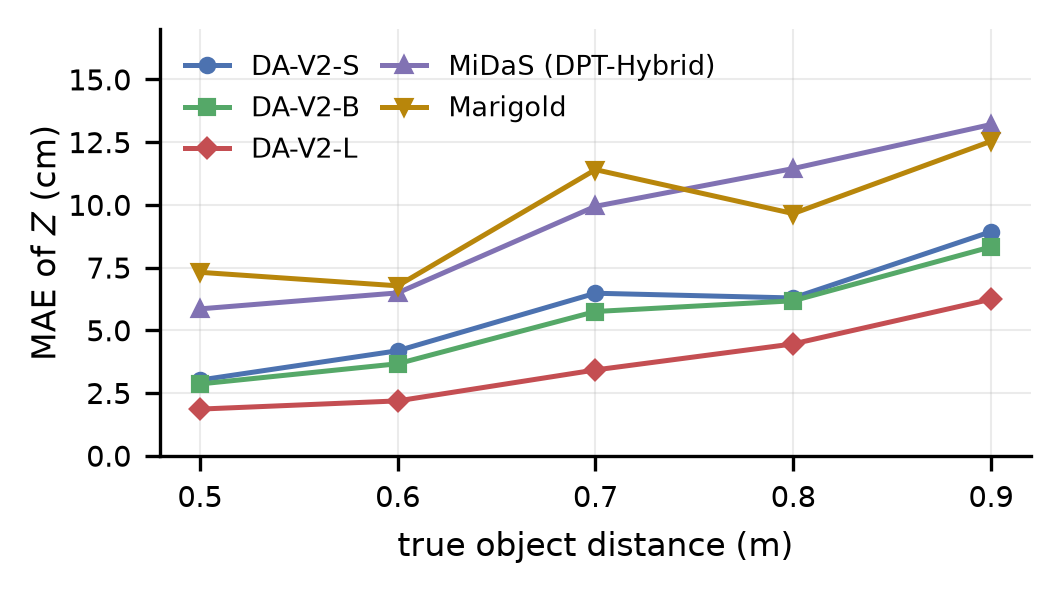
\includegraphics[width=0.80\columnwidth]{fig3_distance.png}
\caption{Mean absolute distance error against true object distance, all objects.
Absolute error grows monotonically for every model but Marigold, while relative
error grows far more slowly (Section~\ref{sec:results}), the signature of a
correctly scaled inverse-depth fit.}
\label{fig:results}
\end{figure}

\subsection{Error Versus Distance}
Figure~\ref{fig:results} shows absolute error growing monotonically with distance
for every model but Marigold. Relative error grows much more slowly, to
about 5--7\,\% for Large, the signature of a correctly scaled inverse-depth fit:
the geometry is sound and the limits are resolution, sampling and model capacity.
The effective range is 0.50--0.80~m, where Large stays under 4.5~cm; nothing
here supports sizing beyond 1~m without closer anchor spacing.



\begin{figure}[t]
\centering
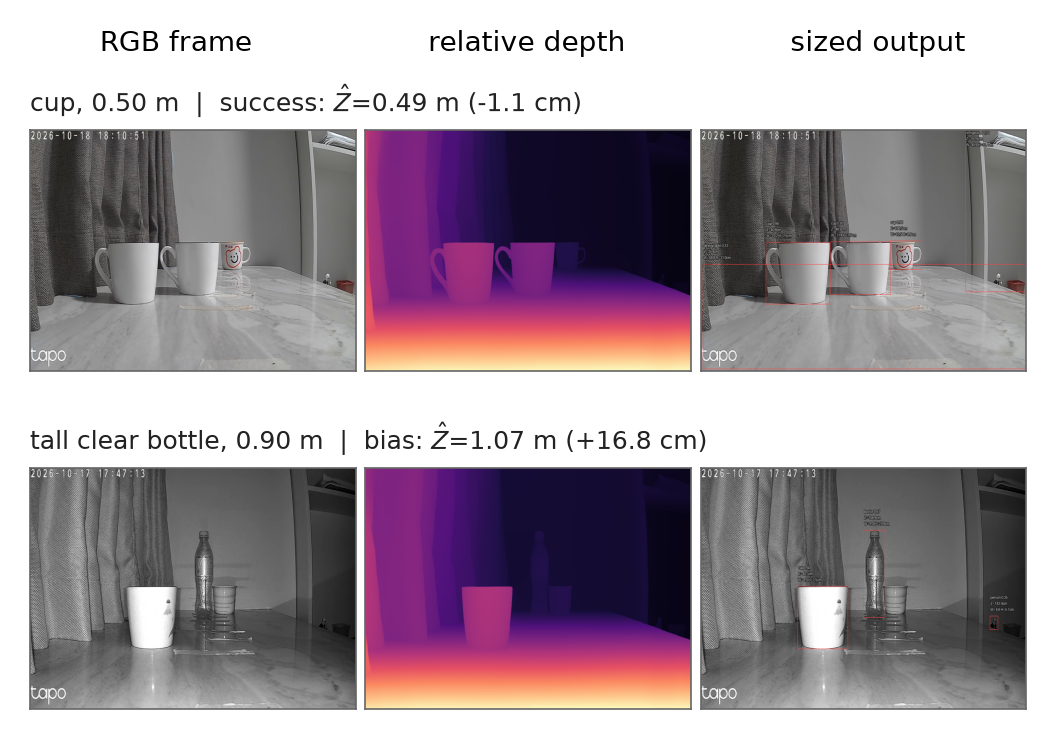
\includegraphics[width=\columnwidth]{fig2_qualitative.png}
\caption{Two frames with Depth Anything V2 Large: a mug at 0.50~m in white light
(top) and the tall clear bottle at 0.90~m under infrared (bottom). Columns
are the RGB input, the relative-depth map (magma, brighter = closer) and the
sized output. The mug is sized to within 1.1~cm; the bottle, which barely
separates from the background in the depth map, is read 16.8~cm too far, and its
width error propagates into a reported 9.1~cm width for a 6.2~cm object.}
\label{fig:qualitative}
\end{figure}

\subsection{The Tall Bottle: A Signed Bias, Not Noise}
\label{sec:b01}
The tall bottle's error is almost entirely one-directional. For Large its MAE of
8.86~cm and its mean signed bias of $+8.86$~cm coincide, so essentially 100\,\%
of the error is over-estimation, and the bias grows with distance, from
$+5.34$~cm at 0.50~m to $+14.05$~cm at 0.90~m. Small is worse in the same
direction, reading a 0.90~m bottle at roughly 1.32~m.

The cause is where depth is sampled, not the depth model; Figure~\ref{fig:qualitative}
shows the case, where the bottle barely separates from the background in the
depth map while the opaque mug pops out. The non-opaque material is a shared
handicap, since the short bottle is translucent and still carries 17.7\,\% of the
total error, but it does not set the magnitude: that bottle stays at 2.5--6.2~cm
for the Depth Anything models, while the tall, colorless one reaches
8.9--20.1~cm.
The difference is silhouette and box tightness. A 24~cm-tall,
6.2~cm-wide object inside a slightly loose box picks up background columns on
both sides; background is farther, so a median over the interior drifts outward.
The tall bottle is also the loosest detection in the set, with confidence down to
0.67. A controlled sweep on the hardest folder confirms the diagnosis: on the
night/tall-bottle images with the Small model and identical anchors, the box
median gives 28.54~cm MAE (39.1\,\%), a box-centre sample 26.12~cm (35.5\,\%),
and a bottom-centre sample 17.03~cm (23.0\,\%). Sampling the ground-contact
point is a 40\,\% cut on the object carrying 61\,\% of the total error, at zero
cost, and it is geometrically the right choice for a standing object because it
is immune to loose horizontal box edges. (That sweep used the default YOLOv8
nano detector, so its absolute level is not comparable with Table~\ref{tab:overall};
the ordering is the result.)

\subsection{Voided Rows and Evaluation Integrity}
\label{sec:integrity}
Of 500 (model, image) pairs, 25 are voided and all 25 are the apple at night:
in every night frame of that folder YOLOv8m returns a cup, a knife, a bowl or a
person, never an apple, so there is nothing to size and those rows are excluded
rather than scored against a substituted object. This matters more than 5\,\%
suggests. An earlier evaluation selected whichever
detection sat most confidently between the anchors, with no class filter, and so
scored calibration cups, knives, bowls and tables in 51 of 500 rows (10.2\,\%).
Those rows averaged 39.5~cm error against 6.5~cm for correctly scored rows and
supplied 60--90\,\% of each model's squared error; one row that sized a knife at
668~cm was 88\,\% of Marigold's total squared error. Correcting it roughly halved
every model's RMSE and changed the object ranking. A pipeline with no
expected-class gate produces plausible, entirely spurious metric errors, and a
per-object breakdown is the cheapest defence.

\section{Limitations}
\label{sec:limits}
\emph{Single camera, assumed intrinsics.} The focal length comes from an assumed
65$^\circ$ horizontal field of view because the device provided no usable EXIF.
Real intrinsics would shift every absolute number, not the relative comparisons.

\emph{One shot per condition.} A single image per cell does not separate model
variance from scene variance.

\emph{Marigold is not reproducible as configured.} The diffusion sampler starts
without a fixed generator or latents and ran at 10 steps with one ensemble member
at 768~px rather than 50 steps and 10 members; its number moved from 17.46 to
8.55~cm between runs, so it should not be quoted as a Marigold result until the
seed and schedule are fixed. It also predicts direct depth rather than disparity,
so \eqref{eq:inverse} does not give it its best case (\eqref{eq:affine} would).
One fit for all models preserves comparability with the earlier run, not fairness
for Marigold.

\emph{Night is confounded with clipping.} Until an exposure bracket is captured,
``depth degrades under infrared'' is not separable from ``this camera clipped the
highlights under infrared''. Tall-bottle folders also use 8$\times$8~cm reference
cups where all others use the 12$\times$8~cm pair; both act only as the 0.40~m
and 1.00~m constants, so the geometry is identical but the scenes are not.

\section{Conclusion and Future Work}
A frozen detector, a frozen depth model and two clicked anchors recover object
dimensions from one RGB frame with useful accuracy: Depth Anything V2 Large
reaches 3.63~cm mean distance error and 9.3\,\% / 4.9\,\% width / height error
across 100 images spanning four lighting conditions, with no gross failures. The
aggregate alone is misleading: bowl and mug sizing is essentially solved at
1--2\,\%, while one tall clear bottle contributes 61\,\% of the total
error, and that error is a signed, distance-growing bias caused by sampling
inside a loose box rather than by a depth failure. Night-time behaviour is
limited by clipped highlights, and honest evaluation requires voiding rows where
the subject is never detected.

Future work follows directly: make bottom-centre sampling the default and
re-run the matrix; apply one scale correction fitted on the anchors to remove the
consistent $+4$ to $+7\,\%$ over-estimation; tighten boxes on the two bottle
classes; and re-run Marigold with a fixed seed and the affine fit, with
bounded-exposure night captures to separate clipping from any inherent
limitation.



\begin{thebibliography}{15}
\bibitem{eigen2014depth}
D.~Eigen, C.~Puhrsch, and R.~Fergus, ``Depth map prediction from a single image
using a multi-scale deep network,'' in \emph{Proc. NIPS}, 2014.

\bibitem{ranftl2022midas}
R.~Ranftl, K.~Lasinger, D.~Hafner, K.~Schindler, and V.~Koltun, ``Towards robust
monocular depth estimation: Mixing datasets for zero-shot cross-dataset
transfer,'' \emph{IEEE Trans. Pattern Anal. Mach. Intell.}, vol.~44, no.~3,
pp.~1620--1634, 2022.

\bibitem{ranftl2021dpt}
R.~Ranftl, A.~Bochkovskiy, and V.~Koltun, ``Vision transformers for dense
prediction,'' in \emph{Proc. ICCV}, 2021.

\bibitem{yang2024da}
L.~Yang, B.~Kang, Z.~Huang, X.~Xu, J.~Feng, and H.~Zhao, ``Depth anything:
Unleashing the power of large-scale unlabeled data,'' in \emph{Proc. CVPR}, 2024.

\bibitem{yang2024dav2}
L.~Yang, B.~Kang, Z.~Huang, Z.~Zhao, X.~Xu, J.~Feng, and H.~Zhao, ``Depth
anything V2,'' in \emph{Proc. NeurIPS}, 2024.

\bibitem{ke2024marigold}
B.~Ke, A.~Obukhov, S.~Huang, N.~Metzger, R.~C. Daudt, and K.~Schindler,
``Repurposing diffusion-based image generators for monocular depth estimation,''
in \emph{Proc. CVPR}, 2024.

\bibitem{bhat2023zoedepth}
S.~F. Bhat, R.~Birkl, D.~Wofk, P.~Wonka, and M.~M{\"u}ller, ``ZoeDepth:
Zero-shot transfer by combining relative and metric depth,''
\emph{arXiv:2302.12288}, 2023.

\bibitem{yin2023metric3d}
W.~Yin \emph{et al.}, ``Metric3D: Towards zero-shot metric 3D prediction from a
single image,'' in \emph{Proc. ICCV}, 2023.

\bibitem{redmon2016yolo}
J.~Redmon, S.~Divvala, R.~Girshick, and A.~Farhadi, ``You only look once:
Unified, real-time object detection,'' in \emph{Proc. CVPR}, 2016.

\bibitem{jocher2023yolov8}
G.~Jocher, A.~Chaurasia, and J.~Qiu, ``Ultralytics YOLOv8,'' 2023. [Online].
Available: \url{https://github.com/ultralytics/ultralytics}

\bibitem{geiger2012kitti}
A.~Geiger, P.~Lenz, and R.~Urtasun, ``Are we ready for autonomous driving? The
KITTI vision benchmark suite,'' in \emph{Proc. CVPR}, 2012.

\bibitem{silberman2012indoor}
N.~Silberman, D.~Hoiem, P.~Kohli, and R.~Fergus, ``Indoor segmentation and
support inference from RGBD images,'' in \emph{Proc. ECCV}, 2012.

\bibitem{hartley2004mvg}
R.~Hartley and A.~Zisserman, \emph{Multiple View Geometry in Computer Vision},
2nd~ed. Cambridge, U.K.: Cambridge Univ. Press, 2004.

\end{thebibliography}

\end{document}
